\section{Waves in Media: Deriving Snell's Law}

%By Matt Trawick, 12/2017

\makelabheader %(Space for student name, etc., defined in master.tex)

\bigskip
\textbf{Activity 1: Making Light Slower}

You have already seen that light is an electromagnetic wave, with a speed $c$ in vacuum given by
$$c = \frac{1}{\sqrt{\epsilon_0 \mu_0}}=3 \times 10^{8}~{\rm m/s}.$$
The ``$\epsilon_0$'' in the equation above is the ``permittivity of free space'', which basically tells you the relationship between charge and electric field in a vacuum.  But suppose the electromagnetic wave is traveling in a clear, dielectric material like water or glass, with a dielectric constant $\kappa$.  (Remember, $\kappa$ is a dimensionless constant always greater than 1.)  In that case, the $\epsilon_0$ in the equation above gets replaced by the permittivity $\epsilon$ of that specific material, given by $\epsilon = \kappa\epsilon_0$.  This changes the speed of electromagnetic waves in that material!

\iflabelexists{deriving_em_waves}
{If you did Lab~\ref{deriving_em_waves}, you can see exactly where the change in speed comes from.  In part~(c) of activity~2 (page~\pageref{part_ampere_field_between_plates}), the electric field between the capacitor plates gets reduced by a factor $1/\kappa$.  The constant $\mu_0\epsilon_0$ you find for Amp\`ere's law becomes $\mu_0\kappa\epsilon_0$ instead, and the extra factor of $\kappa$ carries through the rest of activities~3 and 4 as well.}
{}

\begin{enumerate}[labparts]

\item Inside a dielectric material, or ``medium'', would the speed $v$ of the electromagnetic wave be \textit{faster} or \textit{slower} than in vacuum?
\answerspace{0.4in}

\item The speed $v$ of light in a dielectric material is often expressed as 
$$v = \frac{c}{n},$$
where $n$ is the ``index of refraction'' of the material.  Write an expression below for $n$, in terms of the dielectric constant $\kappa$ of the material.\footnote{In fact, if you look up values of $\kappa$ and $n$ for a particular material, you will probably find that their values don't  obey the relationship you found.  That's because the dielectric constant $\kappa$ depends on the \textit{frequency} of an alternating electric field.  Values of $\kappa$ are usually given for very low frequencies or DC, and values for $n$ are given for the extremely high frequencies of visible light.}
\answerspace{0.6in}

\begin{minipage}{0.70\textwidth}
\item Suppose an electromagnetic wave starts out in a ``fast medium'' like air or vacuum, and then enters a ``slow medium'' like water or glass.  We know that in both regions, the wavelength $\lambda$ and the frequency $f$ are related by $v=f\lambda$.  This means that when the wave enters the slow medium, at least one of two things has to be true: \textit{either} the frequency has to decrease, \textit{or} the wavelength has to decrease.  Which is it, and why?  Make a prediction below.

\textit{Hint: Visualize an analogous situation. Suppose the picture to the right represents waves on the surface of water, traveling from deep water (where waves travel fast) to shallow water (where waves travel slow).  One of the quantities, $f$ or $\lambda$, has to match up between the two regions.  So which one has to decrease?}

\medskip
\hspace{0.5in}Prediction:
\end{minipage}
\begin{minipage}{0.29\textwidth}
\begin{flushright}
\vspace{-0.1in}
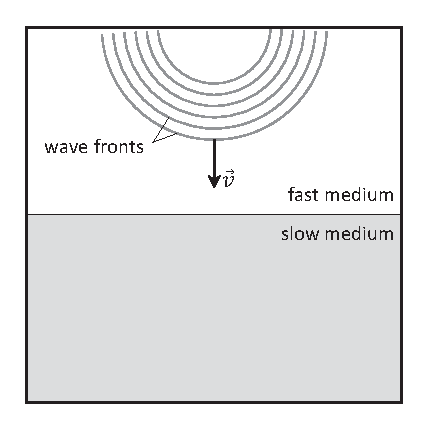
\includegraphics[scale=0.70]{deriving_snells_law/wave_speed_lambda.eps}
\end{flushright}
\end{minipage}

\newpage
\item Now let's test your prediction using software that simulates the motion of waves in different media.  Open \textit{Firefox} and go to \verb!http://falstad.com/ripple/Ripple.html! .  In the topmost menu box to the right, select \button{Example: Slow Medium}, which is about halfway down the list.  Based on this simulation, which quantity, $f$ or $\lambda$, actually decreases in the slow medium?  Was your prediction correct?
\answerspace{0.6in}

If you think carefully about the analogy with water waves, it's clear why the frequency $f$ \textit{has} to be the same on both sides of the boundary.  The whole reason that water on the slow side moves up and down in the first place is because it's \textit{following} the water on the fast side.  So the up and down motion of water \textit{just} across the boundary on the slow side \textit{has} to be synchronized with the water just on the fast side.  It wouldn't make any sense for water on one side to go \textit{up} when water right next to it goes \textit{down}!  The frequencies \textit{have} to be the same for the water on both sides to remain synchronized.  Like water waves, it turns out that some components of the electric and magnetic field vectors in electromagnetic waves have to be continuous across the boundary too.

\item Suppose the fast medium and slow medium have  refractive indices $n_1$ and $n_2$ respectively.  Write an equation below that gives the ratio of their speeds, $v_2/v_1$, in terms of $n_1$ and $n_2$.
\answerspace{0.5in}

\item Starting with the expression $\lambda_2=v_2/f$, write an equation for $\lambda_2$ in terms of \textit{only} $\lambda_1$, $n_1$, and $n_2$.  (Hint: express $f$ in terms of $\lambda_1$ and $v_1$.) \label{part_ratio_of_lambdas}
\answerspace{1.0in}

\end{enumerate}
\textbf{Activity 2: Why Does Light Bend?}

In the ripple simulator, go back to the topmost menu box to the right and select the next option on the list, \button{Example: Refraction}.  In this simulation, an \textit{incident} wave hits the boundary between two media again, but this time at an angle instead of head-on.  As before, there are actually two sets of resulting waves: a \textit{reflected} wave that bounces back into the first medium, and a \textit{refracted} wave that continues into the second medium. 

\begin{enumerate}[labparts]

\item The diagram below shows the velocity vectors of the incident and reflected waves, $\vec{v}_1$ and 
$\vec{v}\,_1'$.  Draw and label a third vector $\vec{v}_2$ on the diagram representing the refracted wave, placing its tail at the head of $\vec{v}_1$.

\begin{center}
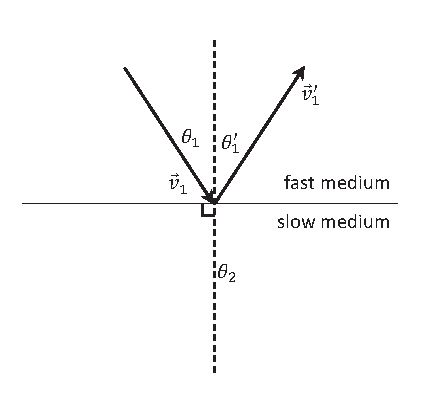
\includegraphics{deriving_snells_law/wave_vectors.eps}
\end{center}
\newpage

\item For all three velocity vectors, the angles between each one and the dotted normal (perpendicular) line are $\theta_1$, $\theta_1'$, and $\theta_2$.  Of the last two, one of them is \textit{exactly equal} to $\theta_1$, and one is \textit{clearly smaller} than $\theta_1$.  Look carefully at the simulation.  Which is which?  Write the two relationships below (using ``$=$'' and ``$<$'') and be sure the previous drawing clearly shows those relationships.
\answerspace{0.4in}

\end{enumerate}

\begin{wrapfigure}[14]{r}{0.42\textwidth}
\begin{flushright}
\vspace{-0.2in}
{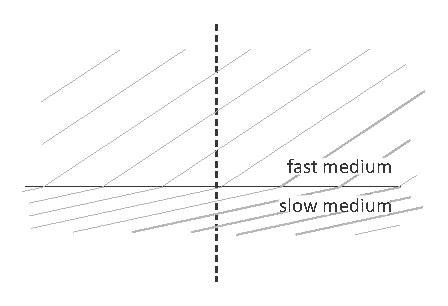
\includegraphics{deriving_snells_law/wave_fronts.eps}}
\end{flushright}
\end{wrapfigure}

The diagram to the right shows the traveling wave fronts of the incident wave and the refracted wave in the two media.  (The reflected wave is left out, for clarity.)  If you think about water waves again, you can see exactly why the directions of the waves \textit{have} to be different on the two sides---it's to make the wave fronts line up with each other along the boundary.  Since the wavelengths are different, if the refracted wave \textit{didn't} change directions in the slow material, the wave fronts on either side of the boundary wouldn't line up: water on one side would be going \textit{up} while water right next to it was going \textit{down}, which wouldn't make any sense!  Again, it turns out that the wave fronts have to line up for electromagnetic waves too, to keep some components of the electric and magnetic fields vectors continuous across the boundary.

\bigskip
\textbf{Activity 2: Deriving Snell's Law}

\begin{minipage}{0.44\textwidth}

Now let's derive an expression to quantify exactly how much light ``bends'' when it goes through two materials with different refractive indices.  The diagram to the right shows a closeup of incident and refracted wave fronts along a boundary.

\begin{enumerate}[labparts]

\item Think about the two triangles in the diagram on either side of the boundary.  One of the interior angles in the upper triangle is equal to $\theta_1$, and one of the interior angles in the lower triangle is equal to $\theta_2$.  Label them.

\item For the wave fronts on both sides to be aligned, the distances $D_1$ and $D_2$ between wave fronts on both sides along the boundary have to be the same.  Rewrite the equation $D_1 = D_2$ in terms of the wavelengths $\lambda_1$ and $\lambda_2$ and the angles $\theta_1$ and $\theta_2$.
\answerspace{0.7in}
\end{enumerate}
\end{minipage}
\begin{minipage}{0.55\textwidth}
\begin{flushright}
\vspace{-0.4in}
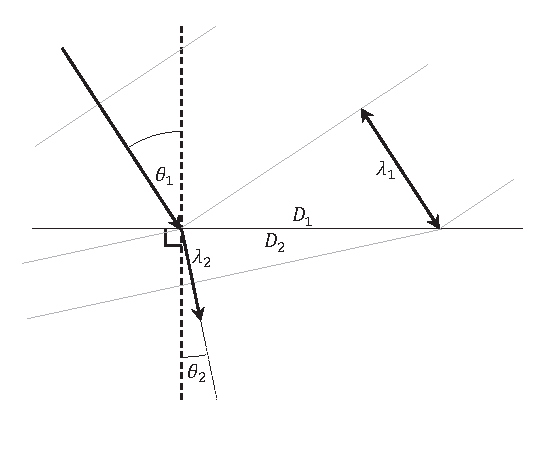
\includegraphics{deriving_snells_law/deriving_snell.eps}
\end{flushright}
\end{minipage}

\begin{enumerate}[labparts,resume]
\item Rewrite your expression in terms of only $n_1$, $n_2$, and the two angles, with no other variables.  (Hint: you can either write each $\lambda$ in terms of $c$, $f$, and $n$, or you can directly use your result from part~\ref{part_ratio_of_lambdas} of activity~1.)
\answerspace{0.8in}
\end{enumerate}
\newpage

The result you just derived is known as Snell's law, and can be applied to lenses and prisms to describe most of what we know about geometric optics, for everything from eyeglasses to telescopes.  It is usually written as $n_1\sin\theta_1 = n_2\sin\theta_2$.  The relationship has been known by lens makers for centuries, but when James Clerk Maxwell discovered in 1862 that light is actually electromagnetic waves, it was then possible to derive Snell's law starting with the fundamental principles of electricity and magnetism.

